\chapterimage{chapter_head_2.pdf} % Chapter heading image

\chapter{\textcolor{red}{Percepção musical}}


\section{\textcolor{red}(Texturas na música)}
The number of voices in a
piece: monophonic, homophonic, and
polyphonic \cite[pp. 322]{harnum2009basic}.

\subsection{\textcolor{red}{A monodia}}
\cite[pp. 38]{schurmann1989m}

\subsection{\textcolor{red}{A polifonia}}
\cite[pp. 64]{schurmann1989m}
\subsubsection{\textcolor{red}{Polirritmia}}
\cite[pp. 93]{alves2004teoria}

\subsection{\textcolor{red}{A homofonia}}
\cite[pp. 121]{schurmann1989m}




%%%%%%%%%%%%%%%%%%%%%%%%%%%%%%%%%%%%%%%%%%%%%%%%%%%%%%%%%%%%%%%%%%%%%%%%%%%%%%%%
\section{\textcolor{red}{Percepção da métrica na música}}

%%%%%%%%%%%%%%%%%%%%%%%%%%%%%%%%%%%%%%%%%%%%%%%%%%%%%%%%%%%%%%%%%%%%%%%%%%%%%%%%
\subsection{\textcolor{red}{Percepção do pulso}}
\index{Musicalidade!Percepção do pulso}
Pulso


%%%%%%%%%%%%%%%%%%%%%%%%%%%%%%%%%%%%%%%%%%%%%%%%%%%%%%%%%%%%%%%%%%%%%%%%%%%%%%%%
\subsection{\textcolor{red}{Percepção dos tempos}}
\index{Musicalidade!Percepção dos tempos}
Tempos


%%%%%%%%%%%%%%%%%%%%%%%%%%%%%%%%%%%%%%%%%%%%%%%%%%%%%%%%%%%%%%%%%%%%%%%%%%%%%%%%
\subsection{\textcolor{red}{Percepção do tempo forte}}
\index{Musicalidade!Percepção do tempo forte}
Tempo forte ou tempo 1

simples
\begin{itemize}
\item O tempo em que estatisticamente percebemos com maior potencia sonora. 
\item Se conseguimos identificar audivelmente um padrão de repetição ``tchic-tchic tum'', o tum é o tempo forte
\item O tempo em que estatisticamente percebemos que o cantor  coloca o acento da palavra \cite[pp. 149]{medteoria}. 
\end{itemize}

complexos 
\begin{itemize}
\item Se percebemos um ``break'' da música com final de frase musical conclusivo 
(satisfatório, com uma sensação de ponto aparte), então este aconteceu no tempo forte.
\end{itemize}


%%%%%%%%%%%%%%%%%%%%%%%%%%%%%%%%%%%%%%%%%%%%%%%%%%%%%%%%%%%%%%%%%%%%%%%%%%%%%%%%
\subsection{\textcolor{red}{Percepção da métrica}}


A Figura \ref{fig:fluxodancanopulso}.

\begin{figure}[h]
    \centering 
\begin{subfigure}[c]{0.45\textwidth}
\centering 
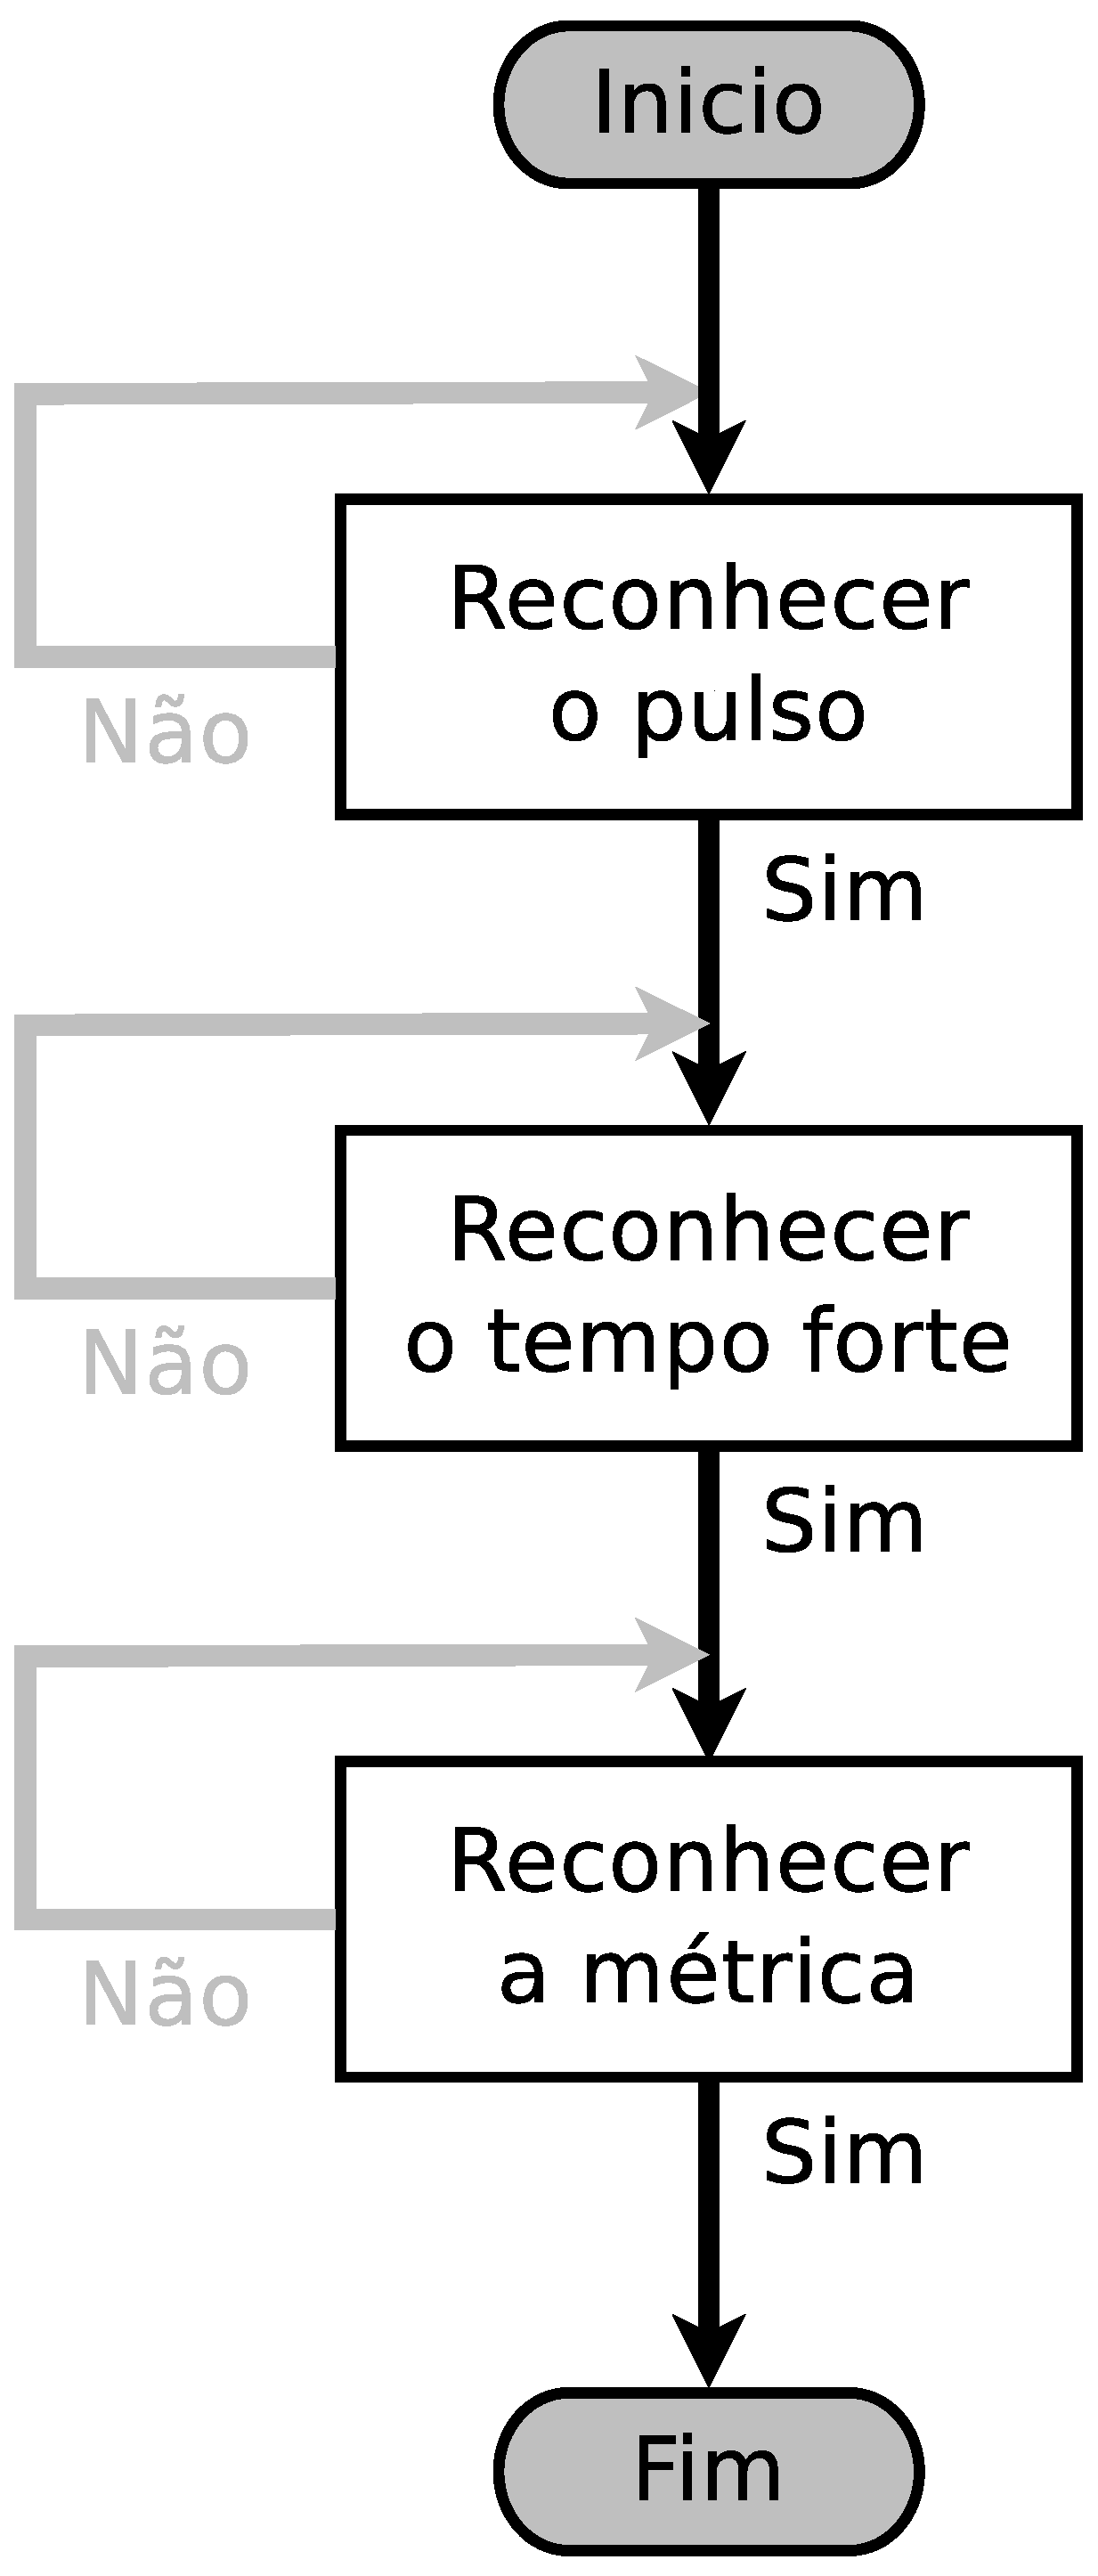
\includegraphics[width=0.6\textwidth]{chapters/cap-musicalidade/dancanopulso1.eps}
\caption{Percebendo a métrica método 1.}
\label{fig:fluxodancanopulso1}
\end{subfigure}
~%
\begin{subfigure}[c]{0.45\textwidth}
\centering 
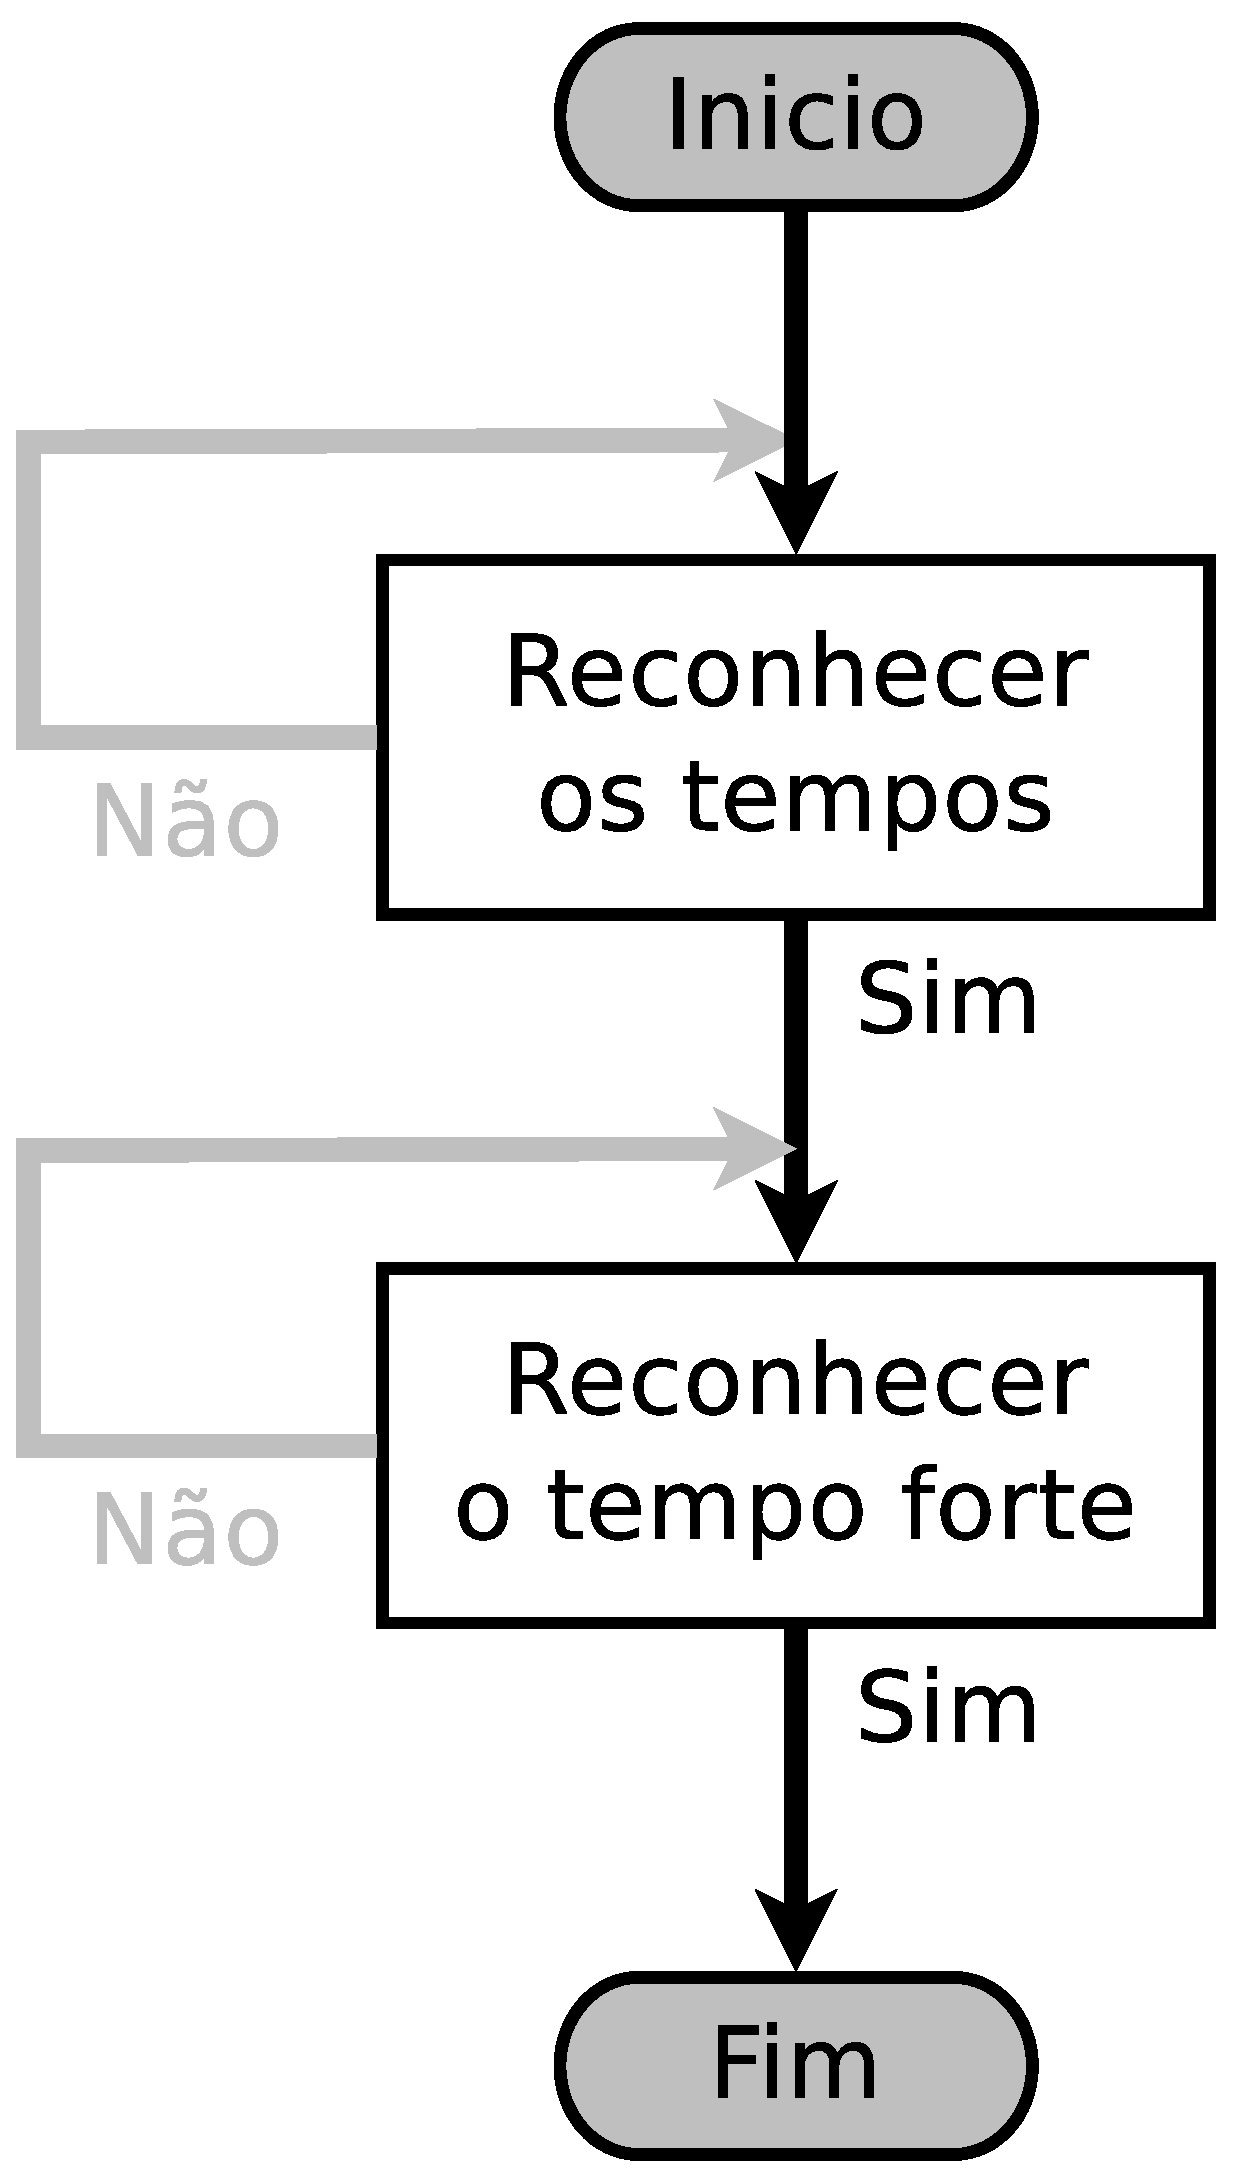
\includegraphics[width=0.6\textwidth]{chapters/cap-musicalidade/dancanopulso2.eps}
\caption{Percebendo a métrica método 2}
\label{fig:fluxodancanopulso2}
\end{subfigure}
    \caption{Percebendo métrica}\label{fig:fluxodancanopulso}
\end{figure}


%%%%%%%%%%%%%%%%%%%%%%%%%%%%%%%%%%%%%%%%%%%%%%%%%%%%%%%%%%%%%%%%%%%%%%%%%%%%%%%%
%%%%%%%%%%%%%%%%%%%%%%%%%%%%%%%%%%%%%%%%%%%%%%%%%%%%%%%%%%%%%%%%%%%%%%%%%%%%%%%%
\section{\textcolor{blue}{Percepção do pulso no samba}}
\index{Musicalidade!Percepção rítmica}
\label{sec:percepcaoouvinte}
Quando escutamos uma música, na qual é tipicamente dançado samba de gafieira,
podemos distinguir que a soma dos sonidos produzidos pelos instrumentos realizam 
um padrão de repetição muito particular, geralmente ligado as onomatopeias: ``tchic-tchic tum'' ou ``tum tum''.


A Figura \ref{fig:abc-caquarela} representa os compassos 18, 19 e 20 da  
composição musical ``Aquarela do Brasil'' escrita
por Ary Barroso em 1939 \cite{AquarelaDoBrasil}; 
a versão mostrada na figura teve arranjos por Irineu Krüger \cite{Irineu}. 
Nesta versão, a música está representada com 1 voz ou coro de voces (``Voice Choir'') e 4 
instrumentos (``Eb'',``Bb'',``Strings'' e ``D. Bass''), que usam uma 
formula de compasso $2/4$, de modo que cada compasso
é binário e
pode ser preenchido usando duas semínimas (2\quarternote).
\begin{figure}[ht]
\centering
%\includegraphics[width=\textwidth]{chapters/cap-fundamentos/aquarela.png}
\begin{abc}[name=abc-caquarela]
% abcm2ps aquarela.abc  -O aquarela.ps
% ps2epsi aquarela.ps aquarela.eps
%
X: 1 % start of header
T: Brazil - Aquarela do Brasil
C: Music: Ary Barroso, 1939
C: Arranged by: Irineu Krüger
K: C % scale: C major
M: 2/4 % formula do compasso
%
V:1 clef=treble name="Voice Choir" sname="Voice Choir"
V:2 clef=treble name="Eb" sname="Eb"
V:3 clef=treble name="Bb" sname="Bb"
V:4 clef=treble name="Strings" sname="Strings"
V:5 clef=bass   name="D. Bass" sname=""D. Bass"
%
%
[V:1] "18" C'3/2A/2C2  |"19" A3/2(G/2 G/2)E1E/2  |"20" z/2 C'1A/2 C'1C'1  |
w:    Ó Bras-sil        sam-ba_ que dá       bam-bo-leio_ 
w:    Ó Bras-sil        ver-de que dá_       pa-ra~o mun-do 
%
%
[V:2] G1z/2G1z/2G1  | G1z/2G1z/2G1  | G1z/2G1z/2G1  |
%
%
[V:3] z4  | z4  | z4  |
%
%
[V:4] G1z/2G1z/2G1  | G1z/2G1z/2G1  | G1z/2G1z/2G1  |
%
%
[V:5] C,2 G,,2  | C,1 z1 G,,2  | C,2 G,,2  |
\end{abc}
\caption{3 compassos da partitura da composição ``Aquarela do brasil''}
\label{fig:abc-caquarela}
\end{figure}

\subsection{Percepção do: tchic-tchic tum}
Analisando este fragmento de partitura e escutando a música produzida, 
podemos perceber que os instrumentos executados em conjunto geram um sonido identificável
com a onomatopeia ``tchic-tchic tum''.
Assim, o inicio de cada compasso coincide com o ``tum''; 
sendo que este é o momento em que a maioria dos instrumentos produzem um sonido, 
de modo que a sensação para o ouvinte é de uma potencia sonora maior. 
Cada instrumento prolongará seu sonido de forma diferente; 
porem,  podemos dizer que: o ``tum'' ocupa $1$ tempo (\quarternote), 
e que o sonido de um ``tchic'' ocupa médio tempo (0.5\quarternote),
sendo que o primeiro ``tchic'' é executado no tempo fraco de ``D. Bass'', 
e o segundo ``tchic'' solapa e obscurece ao  primeiro, 
que é executado na parte fraca do tempo fraco de ``Strings'' ou ``Eb'' (fazendo um contratempo);
conseguindo assim criar a ilusão do ``tchic-tchic tum'', com ``tchic''s de médio tempo ; de modo que:
\begin{equation}
tchic + tchic = tum ~~ \Longleftrightarrow ~~ tchic = \frac{tum}{2}.
\end{equation}
 
Por outro lado, se a percepção do ouvinte é mais
aguçada, poderá escutar ``a tchic-tchic tum''; 
neste caso, o sonido ``tum'' é solapado por o sonido de ``a'',
quando transcorrido um $75\%$ do primeiro tempo do compasso; 
o sonido ``a''  se prolonga incluindo a parte forte do tempo fraco subsequente, 
este sonido é executado pelos instrumentos ``Eb'' e ``Strings'' e constitui uma sincopa \cite[pp. 143]{medteoria}.


Pelo exposto anteriormente, agora podemos simplificar a partitura para gerar um sonido com onomatopeia
``tchic-tchic tum'', como é mostrado na Figura \ref{fig:abc-contratempo1}.
Assim,
o instrumento 1 executa dois sonidos, de modo que o primeiro contribui ao sonido 
``tum'' e o segundo sonido gera o segundo ``tchic'' do compasso; por outro lado,
o instrumento 2 executa um ritmo com um padrão
de repetição de dois sonidos ``tum'' e ``tchic'', nesse ordem;
sendo que a nota executada no tempo forte produz um sonido mais agudo que a 
executada no tempo fraco, isto é assim para poder diferenciar melhor ambos tempos.
\begin{figure}[ht]
\centering
\begin{abc}[name=abc-contratempo1,width=0.75\linewidth]
X: 1 % start of header
K: C % scale: C major
M:2/4
%T: Contratempo num compasso binário
V:1 clef=treble name="Instrumento 1" sname="Inst. 1"
V:2 clef=bass   name="Instrumento 2" sname="Inst. 2"
[V:1] |: " ""T/2"G1 " ""T/2"z1 " ""T/2"z1 " ""T/2"G1 | " ""T/2"G1 " ""T/2"z1 " ""T/2"z1 " ""T/2"G1  :|
w:    tum                tchic                       tum                   tchic           
[V:2] |:  "Tempo"C,2 "Tempo"G,,2  | "Tempo"C,2 "Tempo"G,,2  :|
w:    tum       tchic              tum       tchic            
\end{abc}
\caption{Padrão de repetição para gerar um sonido de onomatopeia ``tchic tchic tum''.}
\label{fig:abc-contratempo1}
\end{figure}

Conhecido tudo isto, é fácil perceber como existe uma diferencia, entre 
o que percebemos ao escutar uma música, e a forma como esta é escrita na partitura;
pois como é visto na Figura \ref{fig:abc-contratempo1}, quando escrevemos
um sonido com um padrão de repetição na ordem ``tum tchic-tchic'', para o ouvinte é mais natural associar
este sonido com o padrão ``tchic-tchic~tum'', devido a que \textbf{quando um ser humano fala, este usa a pausa
para denotar o final de uma palavra}. Da mesma forma, ao escutar uma música, traduzimos
que o sonido que tem um silencio maior apos ser executado marca o final do ciclo
do padrão de repetição. Assim, o que o músico vê ao ler a partitura
é um padrão de repetição ``tum tchic-tchic'', sendo que  um
ouvinte interpretará de forma instintiva que o padrão é ``tchic-tchic tum''.

\subsection{\textcolor{red}{Percepção do: tum~tum}}

Analisando o fragmento de partitura, na Figura \ref{fig:abc-caquarela}, 
e tentando isolar o instrumento ``D. Bass'',
podemos perceber que este gera um sonido identificável com a onomatopeia ``tum tum''.
Podemos ver isoladamente este instrumento, na Figura \ref{fig:abc-contratempo1tumtum}.
\begin{figure}[ht]
\centering
\begin{abc}[name=abc-contratempo1tumtum,width=0.75\linewidth]
X: 1 % start of header
K: C % scale: C major
M:2/4
%T: Contratempo num compasso binário
V:1 clef=bass   name="D. Bass" sname="D. Bass"      
[V:1] |: "Tempo"C,2 "Tempo"G,,2  | "Tempo"C,2 "Tempo"G,,2  :|
w:    tum       tum         tum       tum            
\end{abc}
\caption{Padrão de repetição para gerar um sonido de onomatopeia ``tum tum''.}
\label{fig:abc-contratempo1tumtum}
\end{figure}

%%%%%%%%%%%%%%%%%%%%%%%%%%%%%%%%%%%%%%%%%%%%%%%%%%%%%%%%%%%%%%%%%%%%%%%%%%%%%%%%
%%%%%%%%%%%%%%%%%%%%%%%%%%%%%%%%%%%%%%%%%%%%%%%%%%%%%%%%%%%%%%%%%%%%%%%%%%%%%%%%
\section{\textcolor{blue}{Treinamentos de percepção rítmica}}
\index{Musicalidade!Percepção rítmica}
Nestos exercícios um equipamento ou um professor, 
deve executar uma vez as seguintes sequencias rítmicas, e
seguidamente os ouvintes ou estudantes devem repetir o sonido, 
incluindo as acentuações, primeiro com palmas e logo com os pés.
Nos seguintes exemplos é escrito com maiúscula a onomatopeia 
com acento musical, para lembrar este detalhe na execução do som. 

Percepção do ritmo (TUM tum), a tempo, na Figura \ref{fig:abc-percepcionritmica1}.
\begin{figure}[H]
\centering
\begin{abc}[name=abc-percepcionritmica1,width=0.6\linewidth]
X: 1 % start of header
K: C stafflines=1 % scale: C major
M: 2/4 %meter - compasso
%Q:1/4=80
V:1 clef=perc stem=down %name="Pauta com clave de fá"   sname="Pauta com clave de fá"
[V:1] |: B2  B2| B2  B2 :|  
w: TUM tum TUM tum         
\end{abc}
\caption{Treinamento de percepção rítmica a tempo.}
\label{fig:abc-percepcionritmica1}
\end{figure}

Percepção do ritmo (tum TUM), a contratempo, na Figura \ref{fig:abc-percepcionritmica2}.
\begin{figure}[H]
\centering
\begin{abc}[name=abc-percepcionritmica2,width=0.6\linewidth]
X: 1 % start of header
K: C stafflines=1 % scale: C major
M: 2/4 %meter - compasso
%Q:1/4=80
V:1 clef=perc stem=down %name="Pauta com clave de fá"   sname="Pauta com clave de fá"
[V:1] |: B2  !>!B2| B2  !>!B2 :|
w:      tum  TUM tum TUM   
\end{abc}
\caption{Treinamento de percepção rítmica a contratempo.}
\label{fig:abc-percepcionritmica2}
\end{figure}


Percepção do ritmo (TUM tchic-tchic), a tempo, na Figura \ref{fig:abc-percepcionritmica3}.
\begin{figure}[H]
\centering
\begin{abc}[name=abc-percepcionritmica3,width=0.75\linewidth]
X: 1 % start of header
K: C stafflines=1 % scale: C major
M: 2/4 %meter - compasso
%Q:1/4=80
V:1 clef=perc stem=down %name="Pauta com clave de fá"   sname="Pauta com clave de fá"
[V:1] |: B2  B1 B1| B2  B1 B1 :|
w: TUM tchic tchic TUM tchic tchic      
\end{abc}
\caption{Treinamento de percepção rítmica a tempo.}
\label{fig:abc-percepcionritmica3}
\end{figure}

Percepção do ritmo (tum TCHIC-tchic), a contratempo, na Figura \ref{fig:abc-percepcionritmica4}.
\begin{figure}[H]
\centering
\begin{abc}[name=abc-percepcionritmica4,width=0.75\linewidth]
X: 1 % start of header
K: C stafflines=1 % scale: C major
M: 2/4 %meter - compasso
%Q:1/4=80
V:1 clef=perc stem=down %name="Pauta com clave de fá"   sname="Pauta com clave de fá"
[V:1] |: B2  !>!B1 B1| B2  !>!B1 B1 :|
w: tum TCHIC tchic tum TCHIC tchic         
\end{abc}
\caption{Treinamento de percepção rítmica a contratempo.}
\label{fig:abc-percepcionritmica4}
\end{figure}


Percepção do ritmo (TUM tum-e), a tempo, na Figura \ref{fig:abc-percepcionritmica5}.
\begin{figure}[H]
\centering
\begin{abc}[name=abc-percepcionritmica5,width=0.75\linewidth]
X: 1 % start of header
K: C stafflines=1 % scale: C major
M: 2/4 %meter - compasso
%Q:1/4=80
V:1 clef=perc stem=down %name="Pauta com clave de fá"   sname="Pauta com clave de fá"
[V:1] |: B2  B3/2 B1/2| B2  B3/2 B1/2 :|
w: TUM tum e TUM tum e 
\end{abc}
\caption{Treinamento de percepção rítmica a tempo.}
\label{fig:abc-percepcionritmica5}
\end{figure}

Percepção do ritmo (tum TUM-e), a contratempo, na Figura \ref{fig:abc-percepcionritmica6}.
\begin{figure}[H]
\centering
\begin{abc}[name=abc-percepcionritmica6,width=0.75\linewidth]
X: 1 % start of header
K: C stafflines=1 % scale: C major
M: 2/4 %meter - compasso
%Q:1/4=80
V:1 clef=perc stem=down %name="Pauta com clave de fá"   sname="Pauta com clave de fá"
[V:1] |: B2  !>!B3/2 B1/2| B2  !>!B3/2 B1/2 :| 
w: tum TUM e tum TUM e 
\end{abc}
\caption{Treinamento de percepção rítmica a contratempo.}
\label{fig:abc-percepcionritmica6}
\end{figure}

Percepção do ritmo (TUM tum-e TUM~tchic-tchic), a tempo, na Figura \ref{fig:abc-percepcionritmica7}.
\begin{figure}[H]
\centering
\begin{abc}[name=abc-percepcionritmica7,width=0.75\linewidth]
X: 1 % start of header
K: C stafflines=1 % scale: C major
M: 2/4 %meter - compasso
%Q:1/4=80
V:1 clef=perc stem=down %name="Pauta com clave de fá"   sname="Pauta com clave de fá"
[V:1] |: B2  B3/2 B1/2| B2  B1 B1  :| 
w: TUM tum e TUM tchic tchic   
\end{abc}
\caption{Treinamento de percepção rítmica a tempo.}
\label{fig:abc-percepcionritmica7}
\end{figure}

%\section{Reconhecendo o tom}
% \cite[pp. 116]{alves2004teoria}

